\chapter{Introduction}
\label{cha:introduction}

This chapter introduces the topic area of this thesis as well as the research questions
that this thesis focused on. The topic area of this thesis is introduced in Section \ref{sec:intro_topic}.
The research questions are posed in Section \ref{sec:rq}. Additionally,
this chapter describes the demonstrator project on which this thesis research
was conducted in Section \ref{sec:desc_demonstrator}. This is followed by an overview
of the structure of the thesis in Section \ref{sec:thesis_structure}. The chapter finishes
with a graphic overview of the relationship between the topics discussed in this thesis
in Section \ref{sec:content_overview}.

\section{Introduction to the Topic Area}
\label{sec:intro_topic}

DevOps (Development and Operations) is a philosophy for developing software. It provides practices
and principles which aim to enhance the collaboration between software development and its operation
which in turn should increase the overall efficiency of the software development process.
Today, DevOps and other development processes based on DevOps are widely used in professional environments.
Because of its widespread usage, there is a lot of academic interest in DevOps. Although DevOps focuses
on both the development and operation of software, as its name suggests, most academic research
into the topic only focuses on the development of software including the delivery of software.
Monitoring is a part of operating software systems that has received little attention in academic research.

\begin{quote}
\textit{``Although researchers have focused considerably on build and deployment,
DevOps also impacts infrastructure operations'', \cite{EG+16}}
\end{quote}

This thesis proposes an extension of the UME (Unified Microservice Engineering) approach with a monitoring concept.
The UME approach is a DevOps-based software development process for the development of microservice-based
software by the C\&M (Cooperation \& Management) research group. The main content chapters of this thesis
focus on the development of a monitoring concept for the UME approach, in Chapter \ref{cha:concept},
and its application to a research project from the C\&M group, in Chapter \ref{cha:first_solution}.
The research project that the developed monitoring concept will be applied to is called
BestRentalPoC (BestRental Proof of Concept).
In Subsection \ref{subsec:story} the motivating story of BestRentalPoC is introduced which is later extended
to include the need for a monitoring concept in Chapter \ref{cha:first_solution}.

\subsection*{Story of BestRentalPoC}
\label{subsec:story}

The following is the motivating story behind the demonstrator project BestRentalPoC
(BestRental Proof of Concept) that serves as a concrete project
on which the research of this thesis was conducted.

Alice is a customer of BestRental and has been renting cars from them.
However, every time she rented a car, she had to remember to bring her physical driving license.
Fortunately, DLAKa, the driving license authority in Karlsruhe, 
has introduced a digital driving license option. Alice heard the news and decided to go
to DLAKa to obtain her digital driving license. Bob, who works at DLAKa,
first checks that Alice's physical driving license is valid. Then, Bob fills out a digital form
using the data on Alice's physical driving license. Afterward, Alice scans the QR code on Bob's monitor
using her authenticator app and grants permission to create her digital driving license.
As a result, Alice now possesses a digital driving license in the wallet of her authenticator app.
Alice now can provide digital proof of her valid driving license to anyone who requests it.
Next, Alice rents a car from BestRental. But this time, she uses her digital driving license
to prove that she has a valid one. Once Alice opens the website of BestRental,
she will be prompted to present her digital driving license. Therefore, the website displays a QR Code,
which Alice scans with her authenticator app. Next, Alice confirms the presentation using
her authenticator app and decides what information gets shared. 
Finally, Alice has been verified on BestRental's website and can now rent a car. 
Alice provides the desired period and location for the car rental.
On the website, Alice can then browse and choose from available cars.
Once she has selected a car, BestRental will reserve the car for her.

\section{Research Questions}
\label{sec:rq}

This thesis focuses on developing a monitoring concept that can be integrated into the UME (Unified Microservice Engineering)
approach which is a software development process created by the C\&M (Cooperation \& Management) research group.
The development of the monitoring concept is guided by two research questions that are listed below.
The first research question RQ1 operates on an abstract level and is answered in Chapter \ref{cha:concept}.
The second research question RQ2 takes the results from the first research question and validates them by applying
the developed monitoring concept to the demonstrator project BestRentalPoC (Best Rental Proof of Concept) in Chapter \ref{cha:first_solution}.
An overview of the demonstrator project is given in Section \ref{sec:desc_demonstrator}.

\begin{enumerate}
	\item[RQ1:] How can monitoring be integrated into the UME approach?
	Most research regarding DevOps-based software development processes and practices only focuses
	on the development and deployment of software while leaving out its operation which
	includes monitoring. The UME approach is such a DevOps-based software development process that currently
	does not include a monitoring concept. Extending the UME approach with a monitoring concept is the main goal
	of this thesis.

	\item[RQ2:] How can the adapted UME approach be used to monitor BestRentalPoC?
	The BestRentalPoC is a software project from the C\&M research group that is used
	to test out and develop new engineering practices. This thesis will use this project
	to validate the developed monitoring concept by integrating it into a part of the project.
\end{enumerate}

\section{Description of the Demonstrator}
\label{sec:desc_demonstrator}

The BestRentalPoC is used as a demonstrator in this thesis.
This means that the BestRentalPoC is used to validate the abstract monitoring concept that will be developed
by applying it to a concrete project. The BestRentalPoC consists of three main components: The DLAKaApp, the BestRentalApp,
and Microsoft Entra Verified Id \cite{MIC-ENT}. In its current state, the BestRentalPoC is fully developed but lacks monitoring.
Because the UME approach that was used to develop the BestRentalPoC is based on the DevOps concept, this raises the question
of how monitoring can be integrated into a DevOps-based software engineering process like the UME approach.
This question is answered in Chapter \ref{cha:concept}.

The DLAKaApp consists of the user interface UI-DLAKa (User Interface DLAKa) and the microservice AM-DrivingLicenseManagement
(Application Microservice DrivingLicenseManagement) which are both deployed to a Kubernetes \cite{KUB-DOCS} cluster using Helm \cite{HEL-DOCS}.
The monitoring concept will be applied to the DLAKaApp as an extra component called SPMonitor.
SPMonitor will monitor the issuance of digital driving licenses as well as the resource usage of DLAKaApp's components. 
Because AM-DrivingLicenseManagement is written in the Golang programming language, SPMonitor will need to interact with a microservice
written in Golang and be deployed to a Kubernetes cluster using Helm. The development of SPMonitor can be found in Chapter \ref{cha:first_solution}.

\section{Thesis Structure}
\label{sec:thesis_structure}

The following is a brief overview of the structure of this thesis. Chapter \ref{cha:concept} and \ref{cha:first_solution}
provide the main content of this thesis. The chapters \ref{cha:foundations}, \ref{cha:state_of_the_art}, and
\ref{cha:technical_foundation} provide the knowledge needed by a reader of this thesis.
Chapters \ref{cha:projektteam-arbeiten} and \ref{cha:m2go} describe additional work that was performed
by the author of this thesis that is not related to the research questions posed in Section \ref{sec:rq}.

\subsection*{Chapter 2: Foundations}

Chapter \ref{cha:foundations} contains a brief description of some general concepts
that are necessary for understanding this thesis. The concepts that are described
are decentralized identities, observability and monitoring, DevOps, and CI/CD.

\subsection*{Chapter 3: State of the Art}

Chapter \ref{cha:state_of_the_art} describes some of the research papers that were
used by this thesis. This chapter focuses on the influences of those papers on this
work and the question of whether or not they should be added to the Cooperation and Management
group's literature collection.

\subsection*{Chapter 4: Overall Concept of the Developed Solution}

Chapter \ref{cha:concept} develops the central idea of this thesis: The extension
of the UME approach with a monitoring concept. First, the UME approach,
which employs the DevOps concept, is described. This is followed by an analysis
of how monitoring is used in DevOps. Finally, the extension of the UME approach
by a monitoring concept is explained.

\subsection*{Chapter 5: Technical Foundations}

Chapter \ref{cha:technical_foundation} adds to Chapter \ref{cha:foundations}
by describing concepts that are necessary for the understanding of the solution
that was developed during this thesis but which differ from the concepts in Chapter \ref{cha:foundations}
by being of a more technical nature rather than general concepts.
The technical concepts described in this chapter are containerization, the tool ArgoCD,
and the tools used by the developed solution: Grafana, Prometheus, Grafana Mimir, and MinIO.

\subsection*{Chapter 6: Monitoring DLAKaApp}

Chapter \ref{cha:first_solution} contains the practical application of the concepts
developed in Chapter \ref{cha:concept}. The concept is applied to the microservice
DrivingLicenseManagement of BestRentalPoC. The chapter starts by extending the motivation
for BestRentalPoC to include the need for monitoring. Afterward, the development
of SPMonitor, a tool developed for monitoring BestRentalPoC, is described by going through
the different phases of software development one after another. First, the extended
motivation is analyzed from which use cases are derived that are used to
create requirements and capabilities for SPMonitor. After the analysis,
SPMonitor is designed. The design starts with an abstract software architecture
based on the general requirements for a monitoring tool described in Chapter \ref{cha:foundations}.
This is followed by an API specification for collecting metrics from the microservice DrivingLicenseManagement.
The metrics will be collected from the microservice DrivingLicenseManagement through
the SPMonitor Library.
With the requirements and capabilities as a basis, the tools for SPMonitor are selected next.
Finally, the concrete software architecture of SPMonitor is designed.
The chapter concludes with a description of the implementation and deployment of SPMonitor.

\subsection*{Chapter 7: Organization of the Project Team}

Chapter \ref{cha:projektteam-arbeiten} describes the practical course
that accompanies the WASA2 lecture which is held by the Cooperation and Management group.
During his thesis, the author supervised P3 (project team 3) which was taking
part in the practical course. The tasks of P3 focused on the DevOps side of
BestRentalPoC.

\subsection*{Chapter 8: Contributions to the Practical Course Microservice2Go}

Chapter \ref{cha:m2go} describes the author's contributions to the planning
of a new practical course called Microservice2Go which will be offered by the
Cooperation and Management group alongside the WASA1 lecture, starting in the winter semester
2023/2024. The contributions were focused on the creation of exercises for the implementation part
in the third part of Microservice2Go called Microservice Engineering. This included
developing a microservice implementation which will be used as the template for the exercises.

\subsection*{Chapter 9: Summary and Outlook}

Chapter \ref{cha:outlook} contains the author's summary of this thesis
as well as an outlook on areas of research that require further attention in the future.

\section{Content-related Overview}
\label{sec:content_overview}

Figure \ref{fig:content_overview} illustrates the relationship between the topics
discussed in this thesis. A developer uses the UME (Unified Microservice Engineering) approach
by the C\&M (Cooperation \& Management) group for developing microservice-based software
that uses decentralized identities. Decentralized identities are a method of providing
credentials independent of a central authority based upon decentralization and cryptography.
The UME approach defines a process for developing microservice-based software
using the concepts of DevOps and CI/CD.
The DevOps concept aims to increase the efficiency of software development
through faster product deliveries by taking an agile approach to software development.
CI/CD refers to the practice of continuously delivering new features of software instead
of only delivering the completed software. Containerization provides a method for
deploying software independent of its runtime environment which makes deployments
less complex and reproducible. This thesis extends the UME approach
with a monitoring concept for observing the developed software.
Monitoring collects pre-defined metrics from the software.
Metrics fall into the two categories of technical and business metrics.
Technical metrics relate to the operation and performance of the software.
Examples of technical metrics include the amount of memory used by the software.
Business metrics capture KPIs (Key Performance Indicators) that can be used
by a business to drive business decisions. An example of a business metric
is the usage of a feature.

\begin{figure}[tb]
	\centering
	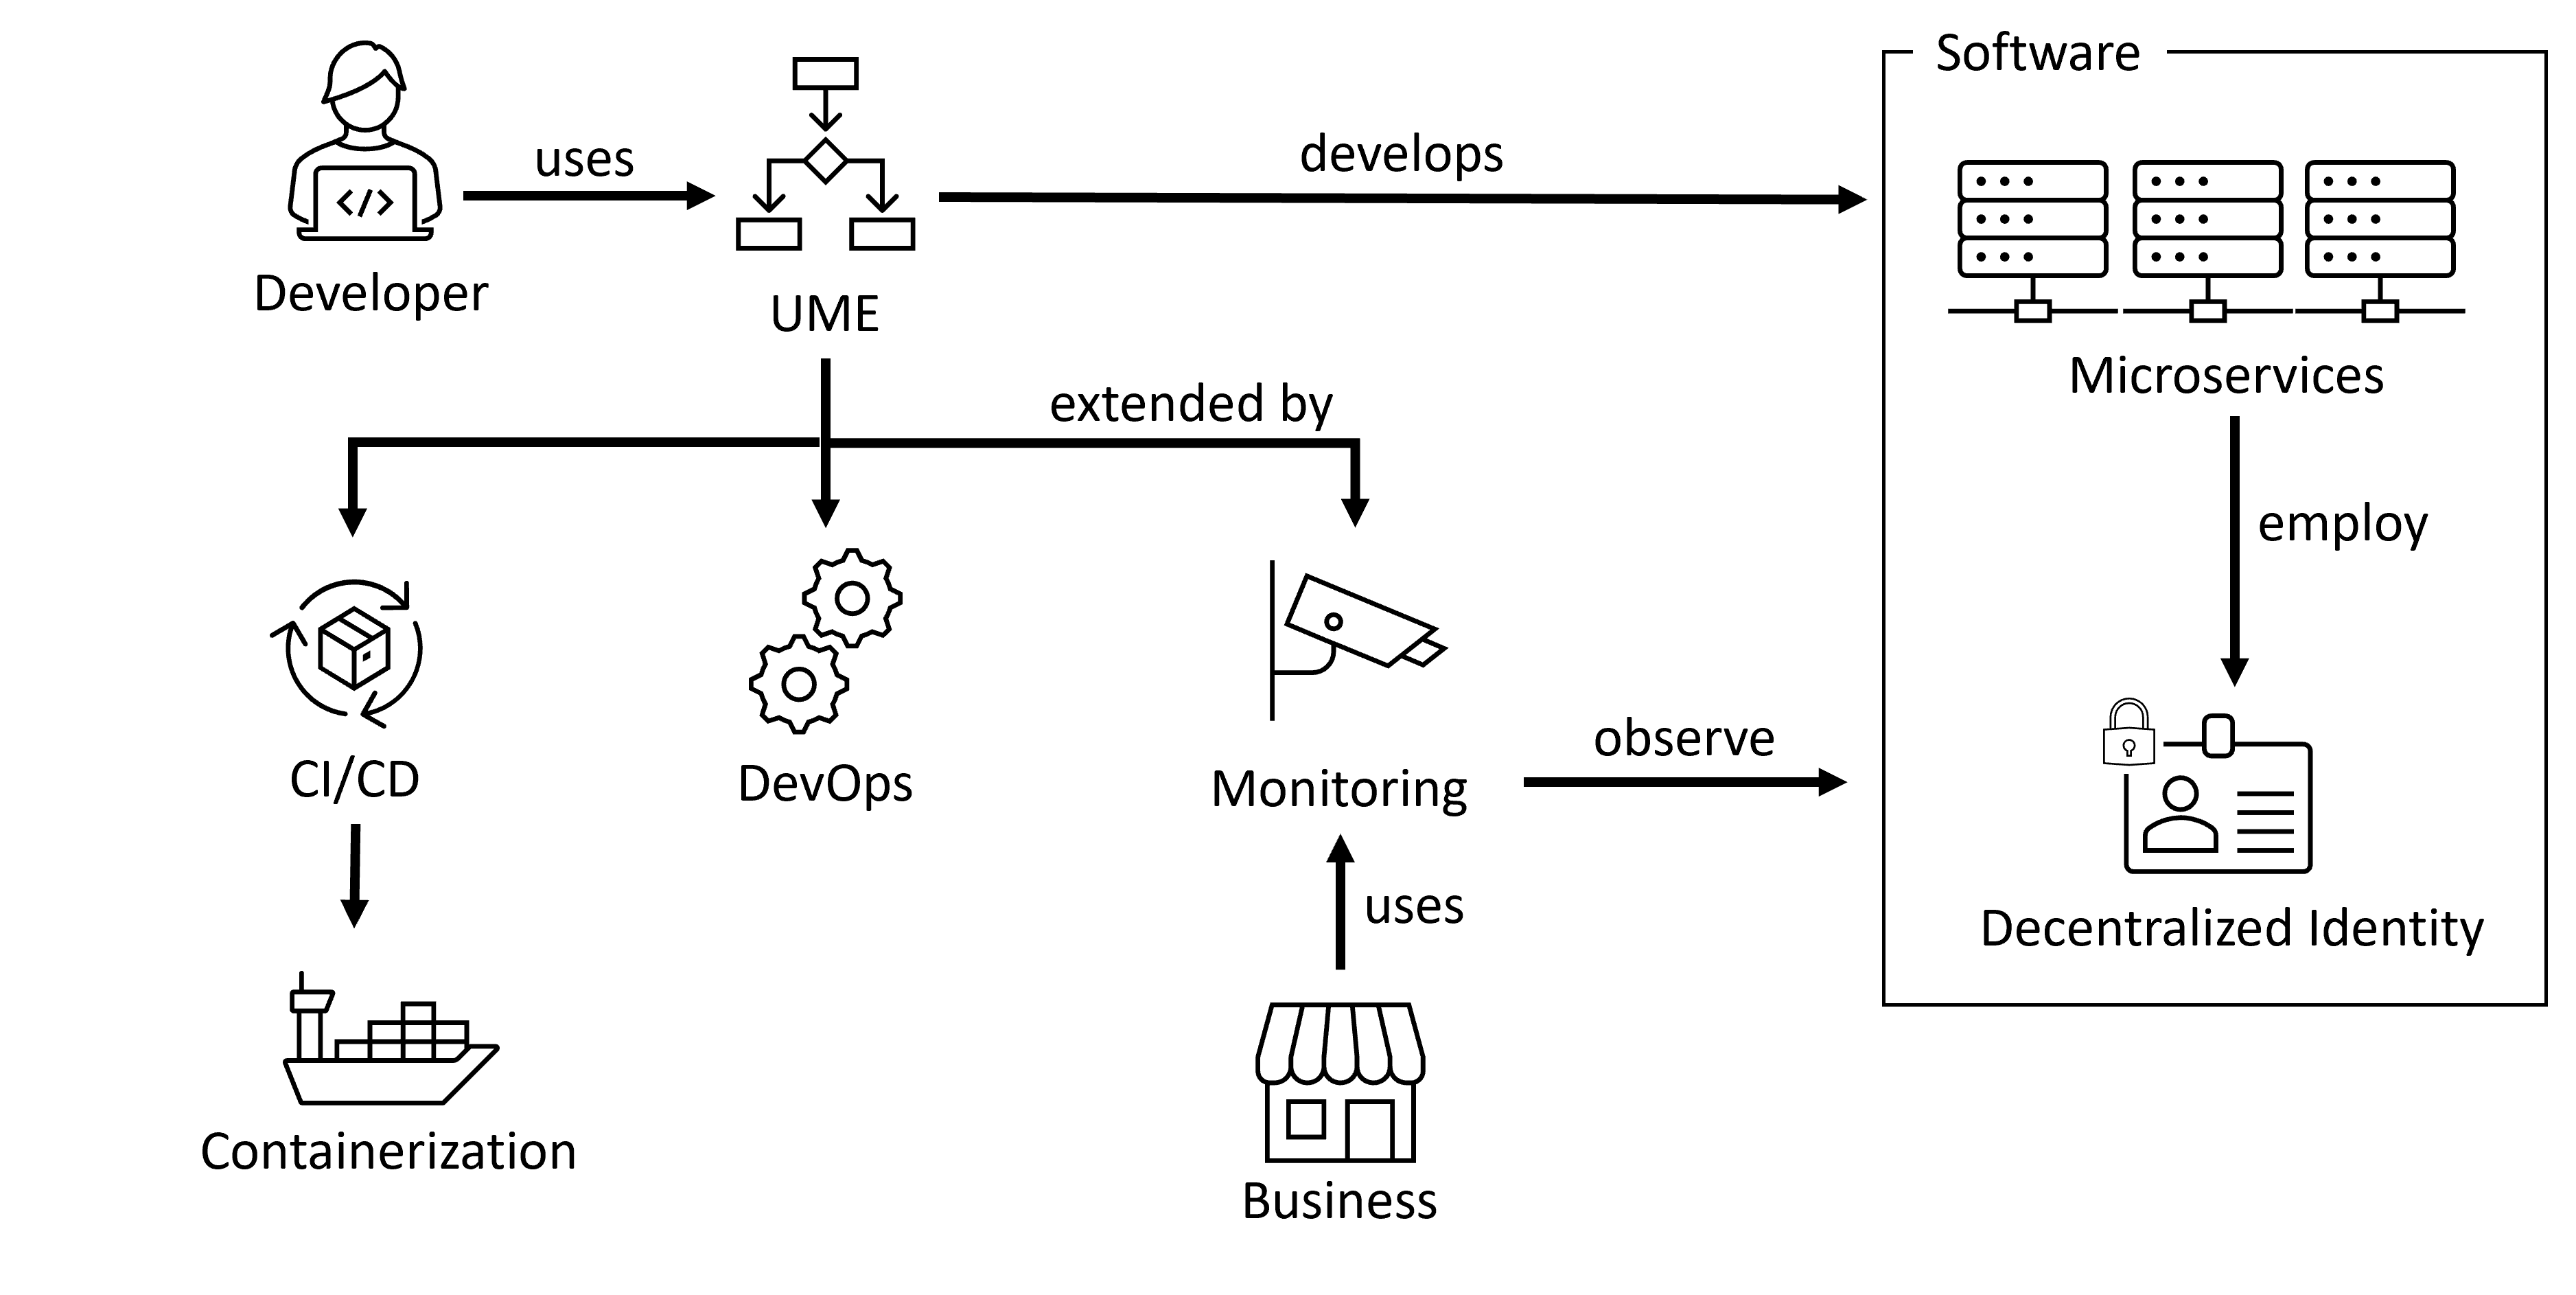
\includegraphics[width=0.7\textwidth]{figures/1.1_content_overview.png}
	\caption{Content-related Overview}
	\label{fig:content_overview}
\end{figure}